\section{Besoins}

Afin de définir les besoins précis du projet, établissons un diagramme bête à cornes puis utilisons de la méthode empirique "QQOQCCP" afin de mieux définir nos attentes.

\begin{figure}[th]
\centering
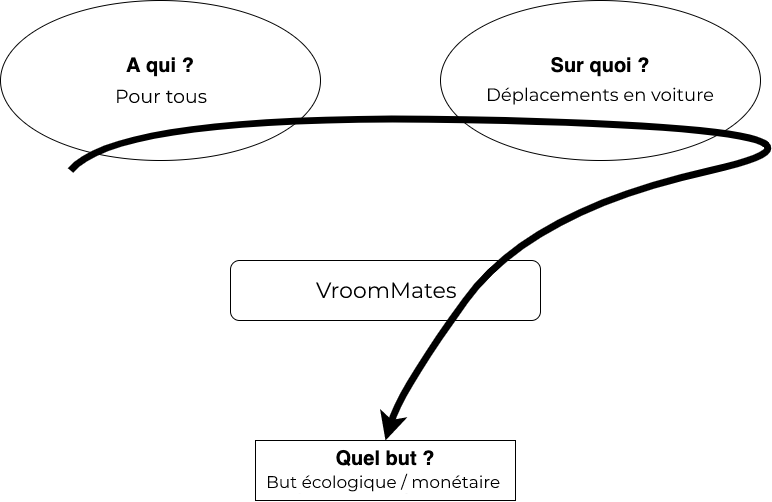
\includegraphics[width=\linewidth]{medias/bete_a_cornes.png}
\decoRule
\caption{Diagramme de bêtes à cornes}
\end{figure}

\paragraph{Pourquoi ?}
Les moyens de déplacement par voiture deviennent de plus en plus problématiques, surtout quand plusieurs personnes vont au même endroit avec une voiture chacun.

\paragraph{Quoi ?}
Nous voudrions offrir une solution de mobilité pour ses utilisateurs qui soit abordable, efficace et inscrite dans une démarche écologique. Nous devons donc mettre en place certains outils, notamment pour la  gestion de projet et d'équipe, afin de résoudre notre problématique de la meilleure façon possible (voir \ref{Outils de gestion de projet et d’équipe}).

\paragraph{Pour qui ?}
Nous voudrions permettre l'utilisation du service au plus grand nombre, sans distinction d'âge, d'origine ou de situation sociale... Cela se ressentira au niveau de notre interface graphique intuitive ainsi qu'à notre politique.

\paragraph{Qui ?}
Les prestataires sont nous-mêmes, le groupe chargé de travailler sur ce projet. Nous avons tout deux les mêmes responsabilités et le même pouvoir décisionnel vis-à-vis du projet.

\paragraph{Où ?}
On remarque cette problématique non seulement en France, mais aussi dans la majorité des autres pays du monde, d'où la nécessité de ne pas se contenter de fournir une solution accessible exclusivement dans l'hexagone.

\paragraph{Comment ?}
Nous allons devoir mettre en place une plateforme Web accessible depuis n'importe quel appareil dit "smart" (téléphone, ordinateur, tablette, ...). Le site sera cependant optimisé pour mobile et ordinateur.
Elle se composera d'un serveur, pour stocker les données(data) et d'une interface Web qui permettra à un utilisateur de se connecter pour commander et/ou de proposer un trajet. On notera aussi l'importance d'avoir un accès administrateur afin de superviser le site.  

\paragraph{Combien ?}
Étant donné la nature du projet (projet étudiant), nous allons devoir réaliser ce travail sans faire recours à des services payants (voir \ref{Contrainte monétaire}).

\paragraph{Quand ?}
Nous avons jusqu'au 05 octobre pour terminer ce projet et le présenter. Un calendrier mis en place sera explicité plus en détail dans les sections à venir (voir \ref{Contrainte de temps}). 
